\section{食宿网行}
    \subsection{校园地图}
   % \paragraph{注}
    \begin{enumerate}
        \item 下面要谈及的重要地点已经用橙色标注出来;
        \item 这份地图版本比较老,图中的西食堂已变为梧桐苑,其西北侧的“拟建大学生文体中心”已建成,我们非常鼓励你去里面健身、打羽毛球、乒乓球等。
    \end{enumerate}
   
   \begin{figure}       
        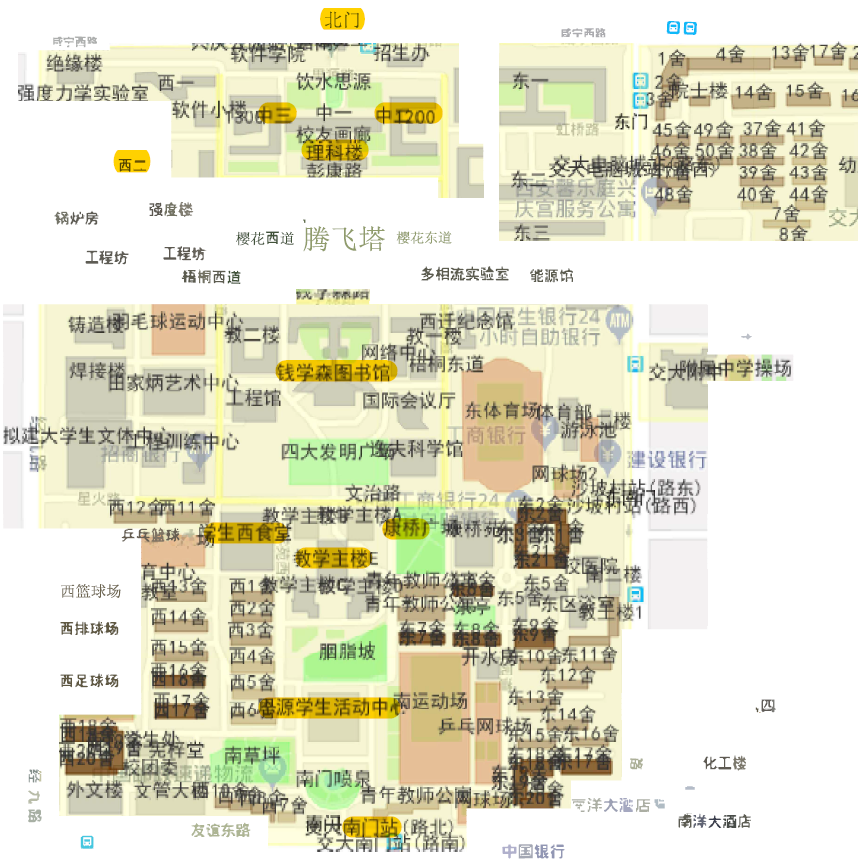
\includegraphics[scale=0.7]{./picture/map.png}     
        \caption{校园地图}
        \label{map}  
    \end{figure}    



    \subsection{饮食}
        \subsubsection{食堂}
            食堂里种类还是蛮丰富的,凭记忆列举必然挂一漏万,所以这里也不求全,这列举大概的品种让你有个初步印象,余下的就请你自己摸索啦!\par
            另外,整体而言,康桥比梧桐便宜一点
            \begin{table}[h]
                \begin{tabular}{c|p{7cm}|p{7cm}}
                    \hline
                    \hline
                         &  康桥   &  梧桐  \\ \hline
                    位置 &  见图\ref{map} &  见图\ref{map} \\ \hline
                    一楼 &  \tabincell{c}{早餐:包子,各种饼,豆浆牛奶,汤圆,\\鸡蛋,粥\\午餐:快餐,各种面,苗香掉渣饼} 
                            & \tabincell{c}{早餐:包子,油条,豆花,豆浆牛奶,粥\\午餐:鸡排饭、砂锅拌饭、黄焖鸡米饭,\\各种面;水吧、果吧}\\ \hline
                    二楼 & \tabincell{c}{自选,各种点心,各种面(有实惠的\\三块七,手头紧张的时候可以缓解经\\济压力)}
                            & \tabincell{c}{自选,各种点心,各种面(有实惠的三\\块五的面),奶茶,饺子}\\ \hline
                    三楼 & \tabincell{c}{各种又贵又好吃的}   & \tabincell{c}{各种又贵又好吃的(清真餐厅、教工\\餐厅、西餐厅)}\\
                    \hline
                    \hline     
                \end{tabular}
                \caption{两个食堂各楼层粗略介绍}
                \label{shitang}
            \end{table}

        \subsubsection{夜宵}
            夜宵出摊的时间不固定,甚至是否出摊也没有规律(主要取决于城管的心情),但一般来说还是建议最早在晚上十点左右去买夜宵;另外,吃夜宵对身体不太好,应少吃哦。
            \begin{enumerate}
                \item 南门:熏肉大饼,杀马特小哥炒细面,烤冷面,炸鸡,烧烤,臭豆腐等等
                \item 东南门:熏肉大饼,小笼包,烧烤,章鱼小丸子等等
            \end{enumerate}

        \subsubsection{聚餐}
            权当抛砖引玉吧,我们也没有去过多少地方。
            \begin{table}
                \begin{tabular}{c|c|p{3cm}|p{3cm}|p{2cm}|p{3cm}}
                    \hline
                    \hline
                          &  店名  &  位置   & 优点   & 缺点   & 备注  \\ \hline
                    炒菜  &  九龙  &  南门口  &  相对便宜,也挺好吃  &  吃多了会腻 & 有烧烤  \\ \hline
                          & 外婆印象 & 东南门外沿北直行,华润万家对面,屈臣氏旁边电梯上二楼 & 相对便宜,好吃 & & 很划算,力荐 \\ \hline
                    风味小吃 &  黄焖鸡米饭  & 南门口  & 挺好吃,有辣度  &  偏贵,人多   &  \\ \hline
                    烧烤  &  老赵烤肉 & 南门一直往南走 &  味道还行 & 偏贵  & \\ \hline
                         &  兰州拉面 & 南门口  & 挺好吃,相对便宜 & 种类偏少  &  \\ \hline
                    自助 &  千家粗粮王 & 东南门外沿北直行,华润万家对面,屈臣氏旁边电梯上三楼 & 相对便宜,也挺好吃 & 吃多了会腻,不适合很多人 &  \\ \hline
                         &  鑫海汇  &  立丰  &  海鲜为主,酒类也较多  &  偏贵  &  \\ \hline
                    火锅 &  重庆老板火锅 & 南门口西行 & 种类多,有辣度,挺好吃 & 贵  & \\ \hline
                         &  龙之秀  & 南门口西行  &  相对便宜,有大包厢  & 店比较小  & 中秋会送月饼,平时也可能会碰上变脸表演\\ \hline
                    串串  &   & 东南门外一条街   & & & \\ \hline    
                \end{tabular}
                \caption{聚餐地点粗略推荐}
                \label{jucan}
            \end{table}

    \subsection{水电费}
    \begin{enumerate}
        \item 找宿管阿姨联系租空调;
        \item 空调电费与其他电费独立,都在康桥一楼西北门的窗口交;
        \item 照明电余量不多(大概还剩五度电)时,宿舍会自动断电,这时找宿管阿姨开电即可,当然要尽快交电费,因为5度电大概只能用2-5天。
        \item 空调电24h供应,熄灯后照明电会断电。
    \end{enumerate}

    \subsection{上网}
    在学校里,上网方式主要分为两种——“宿舍有线网”和“校园Wi-Fi”。为方便起见,我们把宿舍的有线网称为“校园网”。
    \subsubsection{校园网}
    \subsubsection{校园Wi-Fi}
    见表\ref{wifi}
        \begin{table}[h]           
            
            \begin{tabular}{c|c|c|c}
                \hline
                \hline
                名称 & 有信号的地方 & 资费 & 登陆方 + 密码)\\ \hline
                XJTU\_STU & 教学区\footnote{即上课的地方,如主楼、中二、中三等} 及附近的过道 & 20元每月 &netid\verb!@!stu + 校园网密码\\ \hline
                xjtu\_lib  & 图书馆  & 免费  & netid\verb!@!xjtulib + 校园网密码\\ \hline
            \end{tabular}
            
            \caption{校园Wi-Fi}
            \label{wifi}
        \end{table}